\documentclass[11pt,a4paper]{report}

% =============================== PREAMBLE ===============================
\usepackage[utf8]{inputenc}
\usepackage[T1]{fontenc}
\usepackage[margin=2.5cm]{geometry}
\usepackage{amsmath,amssymb,amsthm}
\usepackage{booktabs}
\usepackage{colortbl}
\usepackage{graphicx}
\usepackage{float}
\usepackage{xcolor}
\usepackage{enumitem}
\usepackage{caption}
\usepackage{array}
\usepackage[most]{tcolorbox}
\usepackage[hidelinks]{hyperref}
\usepackage{fancyhdr}
\usepackage{setspace}

\graphicspath{{figures/}}

\definecolor{accent}{RGB}{20,90,60}      % OCP-adjacent institutional green
\definecolor{accent2}{RGB}{40,70,120}
\definecolor{good}{RGB}{30,110,60}
\definecolor{remarkbg}{RGB}{240,246,242}

\hypersetup{colorlinks=true,linkcolor=accent2,urlcolor=accent2,citecolor=accent2}

\pagestyle{fancy}
\fancyhf{}
\lhead{\small Internship Report --- OCP Group}
\rhead{\small\thepage}
\renewcommand{\headrulewidth}{0.4pt}

\newcommand{\keyword}[1]{\textbf{\color{accent2}#1}}
\newcommand{\ours}[1]{{\color{good}\textbf{#1}}}
\newcommand{\code}[1]{\texttt{\small #1}}

\newtcolorbox{remark}[1][Remark]{
  breakable, colback=remarkbg, colframe=accent, coltitle=white,
  fonttitle=\bfseries, title=#1, boxrule=0.6pt, arc=2pt, left=6pt, right=6pt}

% ---------- FILL-IN FIELDS (edit these before submitting) ----------
\newcommand{\StudentName}{El Alami Amine}
\newcommand{\SchoolName}{[Your school / university name]}
\newcommand{\ProgramName}{[Your programme / degree, e.g.\ Engineering degree in Mathematics \& Systems Engineering]}
\newcommand{\AcademicSupervisor}{[Academic supervisor's name]}
\newcommand{\CompanySupervisor}{[Company supervisor's name]}
\newcommand{\InternshipPeriod}{[Start date] -- [End date], 2026}
\newcommand{\HostEntity}{OCP Group --- [host entity / department, e.g.\ Digital \& Information Systems, Cybersecurity]}
% --------------------------------------------------------------------

\begin{document}

% =============================== TITLE PAGE ===============================
\begin{titlepage}
\centering
{\large \SchoolName\par}
{\small \ProgramName\par}
\vspace{0.6cm}
\rule{\textwidth}{0.4pt}\par
\vspace{2.2cm}
{\small INTERNSHIP REPORT / RAPPORT DE STAGE\par}
\vspace{0.8cm}
{\LARGE\bfseries Log Anomaly Detection with Hawkes-Process\\[4pt]
Timing and LLM Triage on System Logs\par}
\vspace{0.6cm}
{\large An unsupervised, rigorously validated pipeline for security-log
analysis,\\ developed during an internship at OCP Group\par}
\vspace{2.2cm}
\begin{tabular}{r p{9.2cm}}
\textbf{Author:} & \StudentName\\[4pt]
\textbf{Host organisation:} & \HostEntity\\[4pt]
\textbf{Company supervisor:} & \CompanySupervisor\\[4pt]
\textbf{Academic supervisor:} & \AcademicSupervisor\\[4pt]
\textbf{Internship period:} & \InternshipPeriod\\
\end{tabular}
\vfill
\rule{\textwidth}{0.4pt}\par
{\small Academic year 2025--2026\par}
\end{titlepage}

% =============================== FRONT MATTER ===============================
\chapter*{Acknowledgements}
\addcontentsline{toc}{chapter}{Acknowledgements}
I would like to express my sincere gratitude to my company supervisor,
\CompanySupervisor, for the guidance, trust, and autonomy granted throughout
this internship, and to the members of the \HostEntity{} team for their welcome
and for the many discussions that helped anchor an academic project in
operational reality. I also thank my academic supervisor,
\AcademicSupervisor, for the methodological guidance and for encouraging the
emphasis placed on rigorous validation. Finally, I thank OCP Group for
providing an environment in which an intern is encouraged to pursue technical
depth, and my professors at \SchoolName{} for the mathematical foundations on
which this work rests.

\chapter*{Abstract}
\addcontentsline{toc}{chapter}{Abstract}
This report documents a two-month internship project carried out within OCP
Group: the design, implementation, and rigorous validation of an end-to-end
anomaly-detection system for machine-generated system logs, augmented with a
stochastic-process model of event timing and a large-language-model (LLM)
triage layer. The system is developed and evaluated entirely on public
benchmark datasets (\code{loghub} HDFS and BGL), which makes every result in
this report reproducible while remaining directly relevant to the
security-operations context of a large industrial group. The pipeline
comprises: (i)~automatic log parsing into structured events (Drain); (ii)~an
unsupervised autoencoder detector benchmarked against an Isolation Forest
baseline; (iii)~a univariate Hawkes point process fitted by maximum likelihood
to model the self-excitation of log events, validated with the time-rescaling
theorem, and evaluated as a source of detection features; (iv)~an adaptive
alerting threshold based on extreme-value theory and a distribution-free
alternative, designed to stabilise the false-alarm rate under distribution
drift; and (v)~an LLM triage agent that deduplicates alerts, correlates them
into incidents, and produces ranked, structured, explained incident reports,
surfaced in a Streamlit dashboard. Validation follows a deliberately strict
protocol: a never-shuffled temporal train/test split, precision--recall
analysis rather than accuracy, a headline metric of false alarms per day at a
fixed detection rate, and explicit measurement of performance drift. Key
results include a detection PR-AUC of $0.987$ on HDFS (a $\sim$20$\times$
reduction in false alarms relative to the baseline), a near-critical Hawkes
branching ratio ($\eta\approx0.97$--$1.0$) on BGL, a measured halving of false
alarms attributable to the timing features, and a demonstrated stabilisation
of the false-alarm rate under drift. Negative and nuanced findings are
reported with the same care as positive ones, as an explicit methodological
choice.

\vspace{0.5em}
\noindent\textbf{Keywords:} anomaly detection, system logs, Hawkes process,
point processes, extreme-value theory, unsupervised learning, autoencoder,
LLM, security operations, OCP.

\tableofcontents
\listoffigures
\listoftables

\chapter*{Acronyms}
\addcontentsline{toc}{chapter}{Acronyms}
\begin{tabular}{@{}ll@{}}
AE & Autoencoder\\
API & Application Programming Interface\\
BGL & Blue Gene/L (supercomputer log dataset)\\
EDA & Exploratory Data Analysis\\
EVT & Extreme-Value Theory\\
FA & False Alarm\\
GPD & Generalized Pareto Distribution\\
HDFS & Hadoop Distributed File System (log dataset)\\
IT / OT & Information Technology / Operational Technology\\
KS & Kolmogorov--Smirnov (test)\\
LLM & Large Language Model\\
MLE & Maximum-Likelihood Estimation\\
MLP & Multilayer Perceptron\\
OCP & OCP Group (historically, Office Ch\'erifien des Phosphates)\\
POT & Peaks-Over-Threshold\\
PR-AUC & Area Under the Precision--Recall Curve\\
SOC & Security Operations Centre\\
UM6P & Mohammed VI Polytechnic University\\
\end{tabular}

% =============================== CHAPTER 1 ===============================
\chapter{General introduction}
\label{ch:intro}

\section{Context of the internship}
This report presents the work carried out during a two-month internship within
\HostEntity. The internship sits at the intersection of two subjects of direct
relevance to a large industrial group: the \emph{operational security} of
digital infrastructure, and the \emph{statistical modelling of event data}.
Modern industrial organisations operate thousands of servers, applications,
and industrial control systems, all of which continuously emit \emph{logs}:
timestamped text records of their activity. These logs are simultaneously the
primary forensic record of the infrastructure and an overwhelming torrent of
data---millions of lines per day---in which the events that matter (failures,
misconfigurations, attacks, cascading faults) are rare, unlabelled, and buried.

The project addresses this problem end to end: it builds a system that ingests
raw logs and produces a short, ranked, explained list of incidents. Beyond the
engineering, the internship had an explicit academic objective, agreed with
both supervisors: to treat the problem as a case study in \emph{rigorous
time-series methodology}---unsupervised learning under class imbalance,
point-process modelling of event timing, extreme-value methods for alerting,
and a validation discipline strict enough to be defensible in front of a
critical audience.

\section{Why this problem matters to OCP}
OCP Group's industrial and commercial operations rest on a large digital
estate (Chapter~\ref{ch:company}). For any organisation of this scale, the
security-operations workload has a well-known structure: monitoring systems
generate far more alerts than analysts can individually review, most alerts
are false or redundant, and genuine incidents manifest as \emph{bursts} of
correlated events rather than isolated signals. The three components of this
project map directly onto that reality: unsupervised detection addresses the
absence of labelled attacks; the Hawkes timing model addresses the bursty,
cascading nature of real incidents; and the triage layer addresses alert
fatigue by converting raw detections into a small number of prioritised,
explained incidents.

\begin{remark}[Scope and data]
For confidentiality and reproducibility, the entire project was developed and
evaluated on \emph{public} benchmark datasets (the \code{loghub} collection:
HDFS and BGL), not on OCP internal data. This was a deliberate design choice
made at the outset: it allows every figure and table in this report to be
reproduced from the accompanying repository, while the methods themselves are
directly transferable to any log source. No internal OCP system, dataset, or
credential was used or is described in this report.
\end{remark}

\section{Objectives}
The objectives fixed at the start of the internship were:
\begin{enumerate}[nosep,leftmargin=1.6em]
  \item Build a complete, reproducible pipeline: raw logs $\to$ structured
  events $\to$ unsupervised detection $\to$ calibrated alerting $\to$ triage
  $\to$ dashboard.
  \item Place a \emph{stochastic-process model} at the mathematical core: fit a
  Hawkes process to event timestamps, estimate its branching ratio, validate
  the fit with the time-rescaling theorem, and evaluate the resulting timing
  features for detection.
  \item Apply a strict validation protocol throughout: temporal train/test
  split, precision--recall analysis, false alarms per day as the headline
  metric, and drift measurement.
  \item Prototype an LLM-based triage agent producing structured, ranked,
  explained incidents, and a dashboard demonstrator.
  \item (Stretch) Investigate extreme-value theory for self-calibrating alert
  thresholds.
\end{enumerate}
All five objectives, including the stretch goal, were completed; the results
are presented in Chapters~\ref{ch:implementation}--\ref{ch:discussion}.

\section{Structure of the report}
Chapter~\ref{ch:company} presents the host organisation, its digital context,
and the positioning of the internship. Chapter~\ref{ch:stateofart} defines the
problem precisely and reviews the state of the art, separating established
prior work from this project's contributions. Chapter~\ref{ch:theory} provides
the theoretical background---each mathematical tool is introduced from first
principles. Chapter~\ref{ch:methodology} describes the methodology: datasets,
system architecture, validation protocol, and engineering practices.
Chapter~\ref{ch:implementation} presents the implementation and results of
every stage, from parsing to the dashboard, including the measurements that
redirected the design. Chapter~\ref{ch:discussion} discusses limitations and
the skills acquired. Chapter~\ref{ch:conclusion} concludes and outlines
perspectives.

% =============================== CHAPTER 2 ===============================
\chapter{Presentation of the host organisation: OCP Group}
\label{ch:company}

\section{Overview and history}
OCP Group (historically \emph{Office Ch\'erifien des Phosphates}) is a
Moroccan public limited company and one of the world's leading producers and
exporters of phosphate rock, phosphoric acid, and phosphate-based fertilizers.
Founded in 1920 to mine the phosphate deposits of the Moroccan plateau, the
organisation has evolved over a century from a mining office into a
vertically integrated industrial group covering the entire phosphate value
chain---extraction, beneficiation, chemical processing, and global
distribution. In 2008 it became a soci\'et\'e anonyme (OCP~S.A.), a
transformation that accompanied a broad programme of industrial modernisation
and internationalisation.

Phosphate is a strategic resource: it is the primary source of phosphorus,
one of the three essential macronutrients in agriculture, and therefore a
cornerstone of global food security. Morocco holds the large majority of the
world's known phosphate rock reserves, and OCP, as their operator, plays a
correspondingly central role both in the national economy---as one of
Morocco's largest companies and export earners---and in the worldwide
fertilizer supply chain, serving customers across the Americas, Europe, Asia,
and, with particular strategic emphasis, Africa.

\section{Industrial footprint}
OCP's operations are organised around integrated mining and processing axes:
\begin{itemize}[nosep,leftmargin=1.6em]
  \item \textbf{Mining sites.} The principal mining basins are
  \emph{Khouribga} (the group's largest), the \emph{Gantour} basin
  (Benguerir and Youssoufia), and \emph{Boucraa}. Ore is extracted,
  beneficiated (washing, flotation, drying), and routed to the chemical
  platforms.
  \item \textbf{Chemical and port platforms.} The \emph{Jorf Lasfar} complex
  on the Atlantic coast---among the largest fertilizer production sites in the
  world---and the \emph{Safi} complex transform phosphate rock into phosphoric
  acid and finished fertilizers for export.
  \item \textbf{The slurry pipeline.} A flagship of the group's modernisation,
  a pipeline of roughly 187~km transports phosphate slurry from Khouribga to
  Jorf Lasfar, replacing rail transport, reducing cost and water/energy
  intensity per tonne, and illustrating the group's strategy of
  infrastructure-led efficiency.
\end{itemize}
Around this industrial core, the group has built an ecosystem of subsidiaries
and partnerships covering engineering, digital technology, research, and
education, discussed below.

\section{Strategy, research, and the skills ecosystem}
Two strategic axes of the group are directly relevant to this internship's
context. The first is \textbf{sustainability}: flagship programmes target the
massive use of desalinated and treated water, large-scale renewable energy for
industrial operations, and ``green'' fertilizer value chains including green
ammonia. The second is \textbf{knowledge and talent}: in 2017 the group
founded \emph{Mohammed~VI Polytechnic University} (UM6P) in Benguerir, a
research university oriented toward applied science, engineering, and
industrial innovation, closely linked to the group's R\&D agenda. Through
UM6P and associated programmes, OCP has positioned itself not only as an
industrial operator but as an anchor of Morocco's scientific and digital
skills ecosystem---the environment in which internships such as this one take
place.

\section{Digital infrastructure and operations}
\label{sec:ocp-digital}
OCP has pursued, over the last decade, a broad \textbf{digital
transformation} of its industrial and corporate operations. Without entering
into internal specifics---which are outside the scope and clearance of this
report---the publicly visible pillars of this transformation, and their
consequences for security operations, can be summarised as follows.

\paragraph{From mine to port: an instrumented value chain.} Modern phosphate
production is heavily instrumented: sensors and industrial control systems
monitor extraction, beneficiation, the slurry pipeline, and chemical
processing. This \emph{operational technology} (OT) estate coexists with a
large corporate \emph{information technology} (IT) estate---enterprise
resource planning, logistics, commerce, engineering, and collaboration
systems. The group has invested in dedicated digital structures and
partnerships to industrialise this transformation, including joint ventures
and entities focused on IT services and digital innovation (for example, a
joint venture with IBM---Teal Technology Services---created to support the
group's IT modernisation, and digital innovation structures associated with
UM6P).

\paragraph{Why this creates a log-analysis problem.} Every layer of such an
estate---servers, network equipment, applications, industrial gateways,
security appliances---continuously emits logs. At industrial scale this
means, conservatively, millions of log lines per day, in heterogeneous
formats, with no labels indicating which lines matter. Security and
reliability teams face three structural difficulties, none specific to OCP but
all amplified by scale:
\begin{enumerate}[nosep,leftmargin=1.6em]
  \item \textbf{Volume asymmetry}: the events worth human attention are a
  vanishing fraction of the stream ($10^{-3}$ or less), so manual review is
  impossible and naive alerting drowns analysts in false positives.
  \item \textbf{Absence of labels}: new failure modes and attack techniques
  appear continuously; no labelled training catalogue can be exhaustive,
  which pushes the state of the art toward \emph{unsupervised} methods that
  model normality.
  \item \textbf{Temporal clustering}: real incidents are \emph{cascades}---one
  root cause triggers bursts of correlated events across systems. Timing
  structure is therefore informative, yet most deployed tooling treats events
  as independent.
\end{enumerate}
These three difficulties are precisely the three axes of this project
(unsupervised detection; timing modelling; triage/correlation), which is what
makes an academically oriented project directly relevant to the operational
context of the host organisation.

\section{Positioning of the internship}
The internship was hosted in \HostEntity. The role of the intern was to
design, implement, validate, and document the complete prototype described in
this report, working autonomously with regular supervision checkpoints. As
stated above, the prototype was developed on public benchmark data so that
the work is fully reproducible and publishable internally without touching
production systems; the methods, however, were selected explicitly for their
transferability to an industrial SOC context: every component consumes
generic structured logs and produces artefacts (scores, calibrated alerts,
ranked incidents) that map onto the daily workflow of a security-operations
team.

% =============================== CHAPTER 3 ===============================
\chapter{Problem statement and state of the art}
\label{ch:stateofart}

\section{Formal problem statement}
Let a log source emit a stream of raw text lines. After parsing
(Section~\ref{sec:parsing-method}), the stream becomes a sequence of events
$\{(t_i, e_i)\}_{i\geq1}$, where $t_i$ is a timestamp and
$e_i\in\{1,\dots,K\}$ is a categorical \emph{event type} drawn from a finite
vocabulary of $K$ templates. Events are grouped into \emph{units of analysis}
$u$ (sessions or fixed time windows), each with an unknown binary state
$y_u\in\{0,1\}$ (normal/anomalous). The task is: using \emph{no} labels at
training time, learn a scoring function $s(u)\in\mathbb{R}$ such that
anomalous units receive systematically higher scores, then convert scores to
alerts via a threshold whose false-alarm behaviour is controlled, and finally
aggregate alerts into a small set of ranked, explained incidents. Ground-truth
labels are used exclusively for evaluation.

Three properties of the domain constrain any solution: extreme class
imbalance ($\Pr[y_u=1]\sim10^{-3}$--$10^{-1}$ depending on the unit);
non-stationarity (the distribution of normal activity drifts over hours and
days); and temporal clustering of events (incidents are cascades). The
evaluation protocol (Section~\ref{sec:validation-protocol}) is designed
around exactly these three properties.

\section{State of the art}
\label{sec:sota}

\paragraph{Log parsing.} The conversion of free-text lines into a finite
template vocabulary is a mature problem. \keyword{Drain}~\cite{drain} is a
fixed-depth parse-tree algorithm that assigns each incoming line to a
template cluster in a single online pass; it is the de-facto standard,
distributed with per-dataset benchmark configurations in the
\code{logparser} toolkit and evaluated across sixteen datasets in the
\code{loghub} benchmark~\cite{loghub}.

\paragraph{Log anomaly detection.} Classical approaches construct a
per-session \emph{event-count matrix} and apply unsupervised detectors---PCA,
invariant mining, clustering, or Isolation Forest~\cite{iforest}---as
systematised in the \code{loglizer} benchmark~\cite{loglizer}. Deep
approaches model event \emph{sequences}: DeepLog~\cite{deeplog} treats logs
as a language and trains an LSTM to predict the next event, flagging
low-probability continuations; LogAnomaly~\cite{loganomaly} extends this with
template semantics. Autoencoders on count vectors are a standard
unsupervised baseline. On the HDFS benchmark, published methods routinely
attain F1 or PR-AUC in the $0.95$--$0.99$ range; the result is heavily
reproduced.

\paragraph{Point processes.} Hawkes processes~\cite{hawkes} are the canonical
model of self-exciting event streams, with mature estimation theory (maximum
likelihood with the exponential-kernel recursion), simulation
(Ogata thinning~\cite{ogata}), and goodness-of-fit machinery (the
time-rescaling theorem~\cite{timerescaling}). They are standard in
seismology, financial microstructure, and social-media modelling. Their use
as a \emph{feature source} for log anomaly detection is, by contrast,
uncommon: the dominant paradigm discards fine-grained timing entirely.

\paragraph{Adaptive thresholding.} Extreme-value theory---the
Pickands--Balkema--de~Haan theorem and the Peaks-Over-Threshold
method~\cite{pickands}---provides the principled route from anomaly scores to
thresholds with controlled exceedance probability. Its streaming application
to anomaly detection is the SPOT/DSPOT family~\cite{spot}.

\paragraph{LLM-based triage.} The use of large language models to summarise,
classify, and prioritise security alerts is an active but young area, largely
driven by industrial practice; the emerging consensus is that LLMs are most
reliable when constrained to structured output schemas and applied
\emph{after} deterministic reduction (deduplication, correlation) of the
alert volume.

\section{Positioning: prior art versus contribution}
\label{sec:positioning}
Table~\ref{tab:priorwork} states explicitly, for each component, what was
already established and what this project adds. Two points deserve emphasis.
First, the HDFS detection result obtained in this work (PR-AUC $0.987$) is a
\emph{reproduction} of a well-known benchmark outcome; it is claimed here
only as evidence that the pipeline is correctly built, and as the substrate
on which the novel components operate. Second, the project's centre of
gravity is elsewhere: the timing model and its honest evaluation, the
validation protocol, the drift-aware thresholding, and the
correlation-grounded triage.

\begin{table}[H]
\centering
\caption{Prior art versus this project's contribution, by component.}
\label{tab:priorwork}
\small
\renewcommand{\arraystretch}{1.2}
\begin{tabular}{@{}p{2.5cm} p{5.6cm} p{5.8cm}@{}}
\toprule
\textbf{Component} & \textbf{Established prior work} & \textbf{\color{good}Contribution of this project} \\
\midrule
Parsing & Drain, standard configurations~\cite{drain}. & Used unchanged, for comparability. \\
Detection & Count-vector AE / IsoForest on HDFS widely reproduced ($0.95$--$0.99$)~\cite{loglizer,deeplog}. & Reproduced as a validated baseline; the added value is the strict protocol and drift analysis around it. \\
Timing & Hawkes theory and diagnostics mature in other fields~\cite{hawkes,timerescaling}. & Applied to logs: branching-ratio estimation on BGL, time-rescaling validation, and a measured ablation of timing features for detection. \\
Thresholding & EVT/POT theory~\cite{pickands}; SPOT for streams~\cite{spot}. & Implemented and verified; documented failure mode on discrete scores; drift-stabilisation demonstration. \\
Triage & LLM alert summarisation (emerging practice). & Correlation grounded in self-excitation; strict JSON schema; dedup-before-LLM design. \\
Validation & Temporal splits and PR analysis known in principle. & Applied end-to-end without exception; false-alarms/day headline; per-period drift reporting. \\
\bottomrule
\end{tabular}
\end{table}

% =============================== CHAPTER 4 ===============================
\chapter{Theoretical background}
\label{ch:theory}

This chapter presents, from first principles, the mathematical tools used in
the project. The aim is that a reader with a general scientific background
can follow every later chapter without external references.

\section{Evaluation under extreme class imbalance}
\label{sec:theory-metrics}
Let a scored test set contain $P$ anomalous and $N$ normal units with
$P\ll N$. For any threshold on the score, the confusion counts
(TP, FP, FN, TN) define
\[
\text{precision}=\frac{\text{TP}}{\text{TP}+\text{FP}},\qquad
\text{recall}=\frac{\text{TP}}{\text{TP}+\text{FN}}.
\]
\emph{Accuracy} $=(\text{TP}+\text{TN})/(P+N)$ is dominated by TN when
$P\ll N$: a degenerate detector that never alerts attains accuracy
$N/(N+P)\approx1$. It is therefore not reported in this work. Sweeping the
threshold traces the precision--recall curve; its area (\keyword{PR-AUC},
equivalently average precision) summarises ranking quality. Its baseline
value for a random scorer equals the positive rate $P/(P+N)$, which makes it
interpretable under imbalance---unlike ROC-AUC, whose false-positive-rate
axis is normalised by the huge $N$ and therefore compresses precisely the
regime that matters.

Operationally, a security team commits to a detection rate and lives with
the resulting alert volume. The headline metric of this work is therefore
\keyword{false alarms per day at fixed recall}: fix recall at $0.90$, find
the smallest score threshold achieving it, count false positives above the
threshold, and divide by the \emph{actual elapsed duration} of the test
period.

\section{Temporal validation and leakage}
\label{sec:theory-temporal}
A model intended to score \emph{future} data must be evaluated on data that
is strictly in the future of everything it was trained on. Random shuffling
violates this: training and test units become interleaved in time, and the
model implicitly exploits information from the test period (shared regimes,
shared incidents), inflating measured performance---a form of \keyword{data
leakage}. The protocol used throughout this work is a \keyword{temporal
split}: units are ordered by start time; the earliest fraction forms the
training set and the strictly later remainder the test set. The prohibition
extends beyond labels: normalisation constants, feature vocabularies, and
alert thresholds are all computed on training data only.

\section{Unsupervised detectors}
\label{sec:theory-detectors}

\subsection{Isolation Forest}
Isolation Forest~\cite{iforest} exploits the fact that anomalies are ``few
and different.'' An isolation tree recursively partitions the data with
axis-aligned random splits; the number of splits required to isolate a point
into its own cell is small for points in sparse regions and large for points
inside dense clusters. Averaging path lengths over an ensemble of randomised
trees yields an anomaly score. The method is unsupervised, near-linear in
sample size, and a standard baseline for tabular anomaly detection---hence
its role here as the detector to beat.

\subsection{Autoencoders}
An \keyword{autoencoder} is a neural network composed of an encoder
$f_\theta:\mathbb{R}^d\to\mathbb{R}^k$ and a decoder
$g_\phi:\mathbb{R}^k\to\mathbb{R}^d$ with $k\ll d$, trained to minimise the
reconstruction error $\|x-g_\phi(f_\theta(x))\|^2$ over a training corpus.
The bottleneck dimension $k$ prevents the identity mapping; to reconstruct
well, the network must learn the dominant regularities of the training
distribution. When trained \emph{exclusively on normal data}, the network
becomes an accurate reconstructor of normal patterns; inputs from outside
that distribution are reconstructed poorly. The per-unit reconstruction
error is thus a natural anomaly score. Compared with the Isolation Forest,
the autoencoder can capture non-linear correlations between features (here,
co-occurrence patterns of event templates) at the cost of training
complexity and hyperparameters.

\section{Point processes and the Hawkes model}
\label{sec:theory-hawkes}

\subsection{Counting processes and conditional intensity}
A temporal \keyword{point process} is a random set of event times
$0<t_1<t_2<\cdots$; equivalently a counting process $N(t)=\#\{i:t_i\leq t\}$.
Its law can be specified through the \keyword{conditional intensity}
\[
\lambda(t)\;=\;\lim_{\Delta\downarrow0}
\frac{\Pr\bigl[N(t+\Delta)-N(t)=1\,\big|\,\mathcal{H}_t\bigr]}{\Delta},
\]
where $\mathcal{H}_t$ is the history of events before $t$: the instantaneous
event rate given the past. The homogeneous Poisson process is the memoryless
special case $\lambda(t)\equiv\mu$; its inter-event times are i.i.d.\
exponential and its counts in disjoint intervals independent. Log streams
violate memorylessness flagrantly---events arrive in bursts---which motivates
a model in which the past excites the future.

\subsection{The Hawkes process}
The (univariate, exponential-kernel) \keyword{Hawkes process}~\cite{hawkes}
posits
\begin{equation}
\lambda(t)\;=\;\mu+\sum_{t_i<t}\alpha\,e^{-\beta(t-t_i)},
\qquad \mu,\alpha,\beta>0.
\label{eq:hawkes}
\end{equation}
Each event raises the intensity by $\alpha$; the excitation decays
exponentially at rate $\beta$ (characteristic memory $1/\beta$). The process
admits a branching (Galton--Watson) representation: ``immigrant'' events
arrive at rate $\mu$, and each event, of any generation, independently
generates offspring according to the kernel. The expected number of direct
offspring per event is
\begin{equation}
\eta\;=\;\int_0^\infty\alpha e^{-\beta s}\,ds\;=\;\frac{\alpha}{\beta},
\label{eq:branching}
\end{equation}
the \keyword{branching ratio}. By branching-process theory the regime
dichotomy is sharp: $\eta<1$ (subcritical) yields finite cascades and a
stationary process with mean rate $\mu/(1-\eta)$; $\eta\geq1$ yields
explosive, non-stationary behaviour. The branching ratio thus condenses
``how cascade-prone is this stream?'' into one interpretable number.

\subsection{Likelihood and estimation}
For events $\{t_i\}_{i=1}^n$ observed on $[0,T]$, the log-likelihood of a
point process with intensity $\lambda$ is
\begin{equation}
\ell=\sum_{i=1}^n\log\lambda(t_i)-\int_0^T\lambda(s)\,ds.
\label{eq:ll}
\end{equation}
The first term rewards intensity placed where events actually occurred; the
second term is the model's expected total event count and penalises
indiscriminately high intensity. For the exponential kernel the integral is
closed-form,
\[
\int_0^T\lambda(s)\,ds=\mu T+\frac{\alpha}{\beta}
\sum_{i=1}^n\Bigl(1-e^{-\beta(T-t_i)}\Bigr),
\]
and the sum term admits Ogata's linear-time recursion: with
$A_i=\sum_{j<i}e^{-\beta(t_i-t_j)}$,
\begin{equation}
A_i=e^{-\beta(t_i-t_{i-1})}(1+A_{i-1}),\qquad A_1=0,\qquad
\lambda(t_i)=\mu+\alpha A_i,
\label{eq:recursion}
\end{equation}
so the full log-likelihood costs $O(n)$ per evaluation rather than the
$O(n^2)$ of the naive double sum---the property that makes maximum-likelihood
estimation feasible on millions of events. In this work $\ell$ is maximised
over $(\log\mu,\log\alpha,\log\beta)$ (rendering the positivity constraints
implicit) with the L-BFGS-B quasi-Newton method.

\subsection{Goodness of fit: the time-rescaling theorem}
\label{sec:theory-rescaling}
Define the \keyword{compensator} $\Lambda(t)=\int_0^t\lambda(s)\,ds$. The
\keyword{time-rescaling theorem}~\cite{timerescaling} states that if
$\{t_i\}$ is a realisation of the process with conditional intensity
$\lambda$, then the transformed times $\tau_i=\Lambda(t_i)$ form a
homogeneous Poisson process of unit rate; equivalently the rescaled
inter-event increments
\[
\Delta\tau_i=\Lambda(t_i)-\Lambda(t_{i-1})
\]
are i.i.d.\ $\mathrm{Exp}(1)$. This converts model checking into a
one-sample distributional test: compute the $\Delta\tau_i$ under the fitted
model and compare them to $\mathrm{Exp}(1)$ via a quantile--quantile plot and
a Kolmogorov--Smirnov statistic. Systematic departures localise the model
error (e.g.\ an excess of large increments indicates the model over-predicts
activity in quiet periods). Two practical points adopted in this work: the
sample mean of $\Delta\tau_i$ must equal $1$ under a correctly normalised
compensator, providing an independent implementation check; and at
$n\sim10^5$ the KS test has such power that it rejects any parametric model,
so the QQ \emph{shape} and the KS \emph{magnitude}, not the $p$-value, are
the meaningful diagnostics.

\subsection{Simulation: Ogata thinning}
To validate an estimator one needs data with known parameters. Ogata's
thinning algorithm~\cite{ogata} simulates a Hawkes process exactly: given the
current intensity bound $M\geq\lambda(t)$, propose the next event after an
$\mathrm{Exp}(M)$ waiting time and accept it with probability
$\lambda(t)/M$; accepted events update the intensity. In this project,
simulation-based recovery of known $(\mu,\alpha,\beta)$ is a mandatory test
that gates any use of the estimator on real data
(Section~\ref{sec:impl-hawkes}).

\section{Extreme-value theory for thresholds}
\label{sec:theory-evt}
Let $X$ be an anomaly score with distribution function $F$, and let $t$ be a
high threshold. The Pickands--Balkema--de~Haan theorem~\cite{pickands} states
that for a wide class of $F$, the conditional law of the exceedance $X-t$
given $X>t$ converges, as $t$ increases, to a \keyword{Generalized Pareto
Distribution},
\[
\Pr[X-t>x\mid X>t]\;\approx\;
\Bigl(1+\frac{\gamma x}{\sigma}\Bigr)^{-1/\gamma},
\]
with shape $\gamma$ and scale $\sigma$. The \keyword{Peaks-Over-Threshold}
method estimates $(\gamma,\sigma)$ from observed exceedances and inverts the
tail to obtain the level $z_q$ crossed with target probability $q$:
\begin{equation}
z_q=t+\frac{\sigma}{\gamma}\Bigl[\bigl(\tfrac{q\,n}{N_t}\bigr)^{-\gamma}-1\Bigr],
\label{eq:zq}
\end{equation}
where $n$ is the sample size and $N_t$ the number of exceedances above $t$.
Re-estimating $(t,\gamma,\sigma)$ on a trailing window while holding $q$
fixed yields a \emph{self-calibrating} alert threshold that tracks
distribution drift---the streaming construction popularised by
SPOT~\cite{spot}. The theorem's hypotheses matter: it concerns
\emph{continuous} tails, a point that becomes material in
Section~\ref{sec:impl-evt}.

% =============================== CHAPTER 5 ===============================
\chapter{Methodology and system design}
\label{ch:methodology}

\section{Datasets}
\label{sec:method-data}
Two public datasets from the \code{loghub} collection~\cite{loghub} were
used; their complementary properties are summarised in
Table~\ref{tab:datasets} and were themselves the object of measurement
(Section~\ref{sec:impl-eda}).

\begin{table}[H]
\centering
\caption{Datasets and their roles.}
\label{tab:datasets}
\small
\renewcommand{\arraystretch}{1.2}
\begin{tabular}{@{}l l l@{}}
\toprule
 & \textbf{HDFS} & \textbf{BGL} \\
\midrule
Origin & Hadoop Distributed File System & Blue Gene/L supercomputer (RAS log) \\
Raw volume & 11{,}175{,}629 lines & 4{,}713{,}493 lines \\
Time span & $\approx$ 1.6 days & $\approx$ 214.7 days \\
Labels & per \emph{block} (2.93\% anomalous) & per \emph{line} (7.39\% alerts) \\
Timestamps & 1-second resolution & microsecond resolution \\
Role & detection \& triage & Hawkes timing model \\
\bottomrule
\end{tabular}
\end{table}

In HDFS, files are stored as replicated \emph{blocks}; each block's lifecycle
generates a short session of log lines, and ground truth labels each block
Normal or Anomaly. In BGL, each line carries an inline label (\code{-} for
non-alert). The decisive difference is timestamp resolution, whose
consequences are established empirically in Section~\ref{sec:impl-eda} and
drive the assignment of roles.

\section{Pipeline architecture}
\label{sec:method-architecture}
The system is organised as a linear pipeline with two parallel analytical
branches:
\begin{center}
\small
raw logs $\;\to\;$ \textbf{parsing} (Drain) $\;\to\;$ \textbf{features}
$\;\to\;$ \textbf{detection} (AE vs.\ IsoForest) $\;\to\;$
\textbf{thresholding} $\;\to\;$ \textbf{triage} $\;\to\;$ dashboard\\[2pt]
\hspace{4.2cm}$\searrow$ \textbf{Hawkes timing model} (BGL) $\nearrow$
\end{center}
Each stage is a Python module in an installable package
(\code{src/logtriage/}), with one thin runnable script per stage
(\code{scripts/}); every stage reads the previous stage's artefacts from a
data directory and writes its own. This separation ensures that notebooks,
scripts, and the dashboard exercise \emph{identical} logic, and that each
stage is independently testable.

\section{Log parsing}
\label{sec:parsing-method}
Drain was applied with the published benchmark configuration for each dataset
(fixed depth~4, similarity threshold~0.5, dataset-specific masking of
variable tokens such as block identifiers and IP addresses). The output is,
per line: timestamp, template identifier, template string, and
dataset-specific fields (HDFS: the referenced \code{block\_id}s; BGL: the
inline label and the node). Using the standard configuration was a
deliberate methodological choice: it makes the template vocabulary---and
hence all downstream results---comparable with the published literature.

\section{Feature construction}
\label{sec:method-features}
\paragraph{HDFS: block sessions.} Since labels are per block, the unit of
analysis is the \emph{block session}: all lines referencing a given block.
Each session is represented by its \keyword{event-count vector}
$x_u\in\mathbb{N}^{48}$, whose $j$-th entry counts occurrences of template
$j$ in the session. Counts are transformed by $x\mapsto\log(1+x)$ to tame
heavy-tailed template frequencies; for the autoencoder they are further
standardised with moments computed \emph{on normal training data only}.

\paragraph{BGL: fixed windows with content and timing blocks.} BGL has no
natural session key, so the stream is segmented into fixed 60-second
windows. Each window receives two feature blocks: a \emph{content} block
(counts of the top-50 templates, vocabulary fixed on training data), and a
\emph{timing} block derived from the Hawkes machinery---the self-excitation
level $A(t)=\sum_{t_i<t}e^{-\beta(t-t_i)}$ evaluated along the window and
summarised (mean, maximum) at two decay scales ($\beta^{-1}=1$\,s and
$30$\,s), plus the window event count. The timing block uses event
\emph{times only}---never labels---so it is a legitimate feature under the
leakage rules. A window is labelled anomalous if it contains at least one
alert line (evaluation only).

\section{Validation protocol}
\label{sec:validation-protocol}
The protocol, fixed before any model was trained, is:
\begin{enumerate}[nosep,leftmargin=1.6em]
  \item \textbf{Temporal split.} Units ordered by start time; earliest 70\%
  train, latest 30\% test; never shuffled. On HDFS this places the boundary
  at 2008-11-11 06:00:46 (402{,}543 / 172{,}518 blocks).
  \item \textbf{Unsupervised training.} The autoencoder trains on
  \emph{normal training} units only (389{,}428 blocks on HDFS); labels never
  enter training, scaling, or vocabulary construction.
  \item \textbf{Metrics.} PR-AUC for ranking quality; precision and false
  alarms per day at recall $0.90$ for operations; all durations computed
  from actual elapsed test time.
  \item \textbf{Drift.} Every metric is additionally computed on consecutive
  chronological slices of the test period, with thresholds fixed once on the
  full test set (an analyst cannot re-tune hourly).
  \item \textbf{Model-agnostic scoring.} All detectors output scores oriented
  ``higher $=$ more anomalous'' and are evaluated by the same code path.
\end{enumerate}

\section{Engineering and quality practices}
\label{sec:method-engineering}
The project was developed under version control (git) with incremental,
reviewed commits. Correctness of the load-bearing logic is enforced by an
automated test suite (34 tests at the time of writing) covering: the metric
implementations (operating points, false-alarms-per-day on synthetic cases
with known answers), the Hawkes machinery (parameter recovery from simulated
data; time-rescaling accepting a true model and rejecting a false one;
monotonicity of the compensator), the EVT threshold (exceedance-rate control
on simulated stationary and drifting streams), the feature builders, and the
triage logic (deduplication, correlation, ranking). A fixed random seed
policy makes runs reproducible. The principle applied throughout---%
\emph{prove components on synthetic data with known ground truth before
applying them to real data}---is standard practice in quantitative fields
and was treated as non-negotiable here.

% =============================== CHAPTER 6 ===============================
\chapter{Implementation and results}
\label{ch:implementation}

This chapter follows the pipeline from raw data to dashboard. For each stage
it states \emph{what} was built, \emph{why} it was built that way, \emph{how}
it works, and what was measured---including the measurements that forced
design changes.

\section{Data acquisition and parsing}
\label{sec:impl-parsing}
Both datasets were downloaded from the public \code{loghub} mirrors and
parsed with Drain under the benchmark configurations. The full HDFS log
(11.2M lines) parses into \textbf{48} templates; BGL (4.7M lines) into
\textbf{429}. Parsing correctness was verified with a structural invariant:
the HDFS template corresponding to block allocation
(\code{NameSystem.allocateBlock}) must occur exactly once per block, and its
occurrence count ($575{,}061$) matches the number of labelled blocks exactly.
An error at this stage would silently corrupt everything downstream, which
is why an exact invariant was preferred over spot-checking.

\section{Exploratory analysis: measurements that shaped the design}
\label{sec:impl-eda}
Three empirical findings, established before any modelling, redirected the
project; we present them as results in their own right.

\paragraph{Finding 1: strong overdispersion (clustering).} For a homogeneous
Poisson process, the \emph{Fano factor} (variance-to-mean ratio of counts in
fixed intervals) equals~1. Measured on per-minute counts, the Fano factor is
$5.3$ on the HDFS sample and $698$--$2286$ on BGL windows---one to three
orders of magnitude above the Poisson value. Event clustering is thus a
dominant, quantifiable property of both streams, justifying a self-exciting
model \emph{before} any fit (Figure~\ref{fig:eda}, left).

\paragraph{Finding 2: HDFS timestamps cannot support a continuous-time
model.} HDFS records time at 1-second resolution while the stream averages
$\approx80$ events/second. Measured consequences: \textbf{98.8\%} of
consecutive events in the global stream carry identical timestamps; within a
single block, $90.5\%$ of consecutive events still tie; every block's
lifetime is $\leq54$\,s (median $7$\,s) and occupies a median of
$\approx2$ distinct second values. A continuous-time point process requires
a strict event ordering that simply is not present. Injecting artificial
sub-second jitter was considered and \emph{rejected}: the estimated
branching ratio would then measure the jitter, not the system. Consequence:
the Hawkes analysis is carried out on BGL, whose microsecond timestamps
exhibit $0\%$ ties.

\paragraph{Finding 3: the anomaly rate itself drifts.} Under the temporal
split, the training period is $3.26\%$ anomalous and the test period
$2.16\%$: the base rate is non-stationary, foreshadowing the drift
phenomena measured in Sections~\ref{sec:impl-detection}
and~\ref{sec:impl-evt}. Figure~\ref{fig:eda} (right) shows the block-session
size distribution (median 19 events); the upper tail is disproportionately
anomalous, consistent with failing blocks emitting additional retry and
error lines.

\begin{figure}[H]
\centering
\IfFileExists{figures/HDFS_timeline.png}{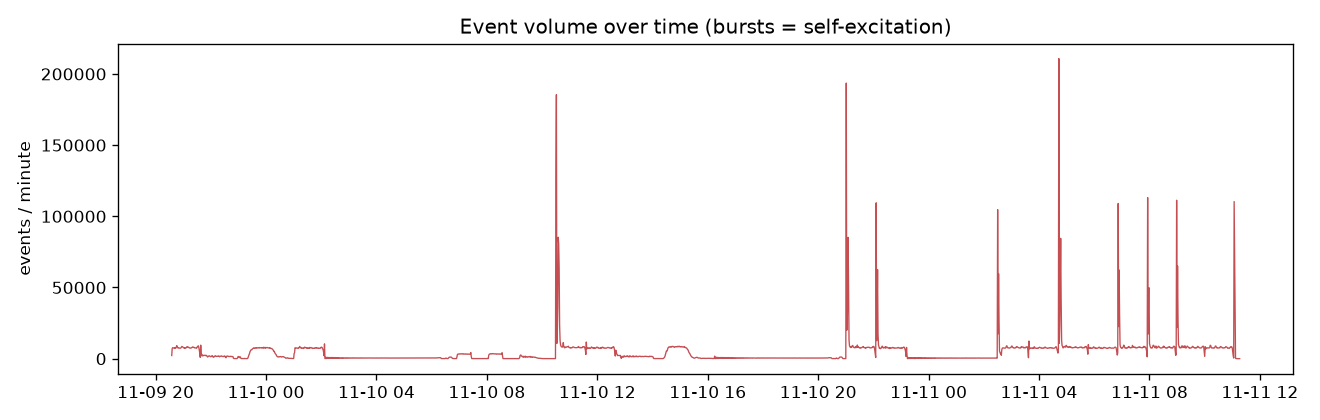
\includegraphics[width=0.49\textwidth]{HDFS_timeline.png}}{\fbox{figure}}
\IfFileExists{figures/HDFS_block_sizes.png}{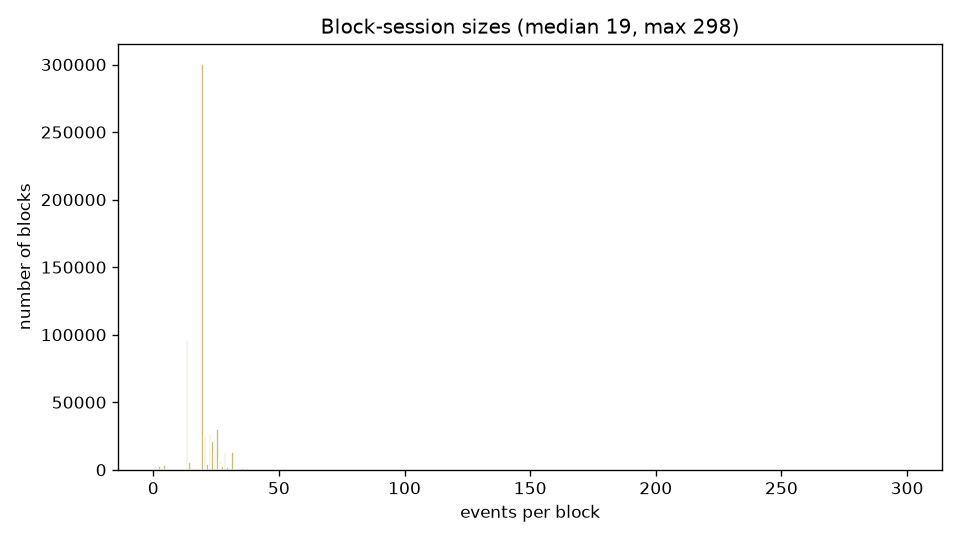
\includegraphics[width=0.49\textwidth]{HDFS_block_sizes.png}}{\fbox{figure}}
\caption{Left: HDFS event volume per minute---a flat baseline punctuated by
bursts, the visual signature of self-excitation. Right: block-session sizes
(median 19, maximum 298).}
\label{fig:eda}
\end{figure}

\section{Detection on HDFS}
\label{sec:impl-detection}

\paragraph{Setup.} Unit: block session; features: 48-dimensional count
vectors (Section~\ref{sec:method-features}); split and metrics as in
Section~\ref{sec:validation-protocol}. The baseline Isolation Forest is fit
on $\log(1+x)$ counts. The autoencoder is a multilayer perceptron
$48\to32\to16\to8\to16\to32\to48$ with ReLU activations, trained with Adam
on normal training blocks only, with early stopping on a held-out slice of
the normal training data (convergence in $\approx19$ epochs); the anomaly
score is the per-block reconstruction mean-squared error.

\paragraph{Results.} Table~\ref{tab:detect} and Figure~\ref{fig:pr}
summarise the test-set outcome.

\begin{table}[H]
\centering
\caption{HDFS detection, temporal test split (172{,}518 blocks, 2.16\%
anomalous).}
\label{tab:detect}
\small
\renewcommand{\arraystretch}{1.2}
\begin{tabular}{@{}l c c@{}}
\toprule
Metric & Isolation Forest & \color{good}Autoencoder \\
\midrule
PR-AUC & $0.748$ & \ours{$0.987$} \\
Precision at recall $0.90$ & $0.556$ & \ours{$0.961$} \\
False alarms / day at recall $0.90$ & $\sim12{,}700$ & \ours{$\sim650$} \\
\bottomrule
\end{tabular}
\end{table}

\begin{figure}[H]
\centering
\IfFileExists{figures/hdfs_pr_comparison.png}{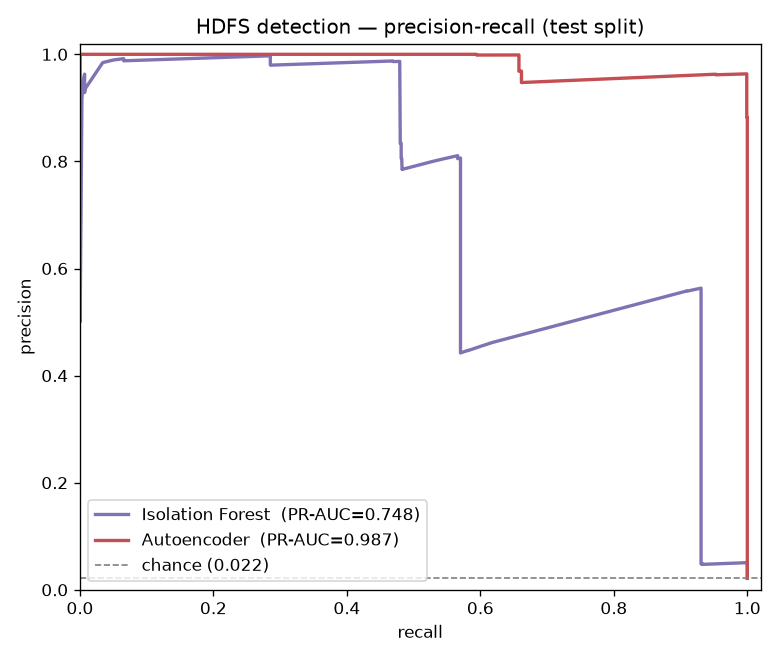
\includegraphics[width=0.6\textwidth]{hdfs_pr_comparison.png}}{\fbox{figure}}
\caption{Precision--recall curves on the HDFS test split. The autoencoder
dominates the baseline at every operating point; the dashed line marks the
chance level (0.022).}
\label{fig:pr}
\end{figure}

At the committed $90\%$ detection rate the autoencoder reduces the
false-alarm burden by a factor of $\approx20$. The drift decomposition adds
an important nuance: across four consecutive slices of the test window, the
baseline's PR-AUC oscillates between $0.69$ and $0.98$, while the
autoencoder holds $\geq0.99$ throughout---its ranking is not merely better
but \emph{stabler}. However, the \emph{false-alarm rate at a fixed
threshold} is not stable even for the autoencoder (it varies by orders of
magnitude across slices), which motivates Section~\ref{sec:impl-evt}.

\begin{remark}[Positioning]
This result reproduces a well-established benchmark outcome
(Section~\ref{sec:positioning}) and is claimed only as validation of the
pipeline. Its role in the project is to supply a trustworthy detector and
realistic anomaly scores to the components that follow.
\end{remark}

\section{The Hawkes timing model on BGL}
\label{sec:impl-hawkes}

\paragraph{Estimator verification.} Before any application to real data, the
estimator was gated by simulation tests: trajectories generated by Ogata
thinning with known $(\mu,\alpha,\beta)$ are refit, and the estimates must
recover the truth (achieved within a few percent); the time-rescaling
diagnostic must accept the true model and reject a deliberately mis-specified
one (both verified). Only then was the estimator applied to BGL.

\paragraph{Fits.} Two contrasting 24-hour windows were analysed: a calm day
(2005-09-03; 6{,}858 events) and a severe fault cascade (2005-06-11;
152{,}669 events). Table~\ref{tab:hawkes} reports the fits;
Figure~\ref{fig:hawkes} shows the fitted intensity and the time-rescaling
QQ-plots.

\begin{table}[H]
\centering
\caption{Maximum-likelihood Hawkes fits on BGL windows.}
\label{tab:hawkes}
\small
\renewcommand{\arraystretch}{1.2}
\begin{tabular}{@{}l c c c c@{}}
\toprule
Window & Events & $\eta=\alpha/\beta$ & KS statistic & mean rescaled gap \\
\midrule
2005-09-03 (calm) & 6{,}858 & $\mathbf{0.971}$ & 0.095 & 1.0001 \\
2005-06-11 (cascade) & 152{,}669 & $\mathbf{0.9998}$ & 0.431 & 1.0000 \\
\bottomrule
\end{tabular}
\end{table}

\begin{figure}[H]
\centering
\IfFileExists{figures/bgl_hawkes_2005-09-03_all_intensity.png}{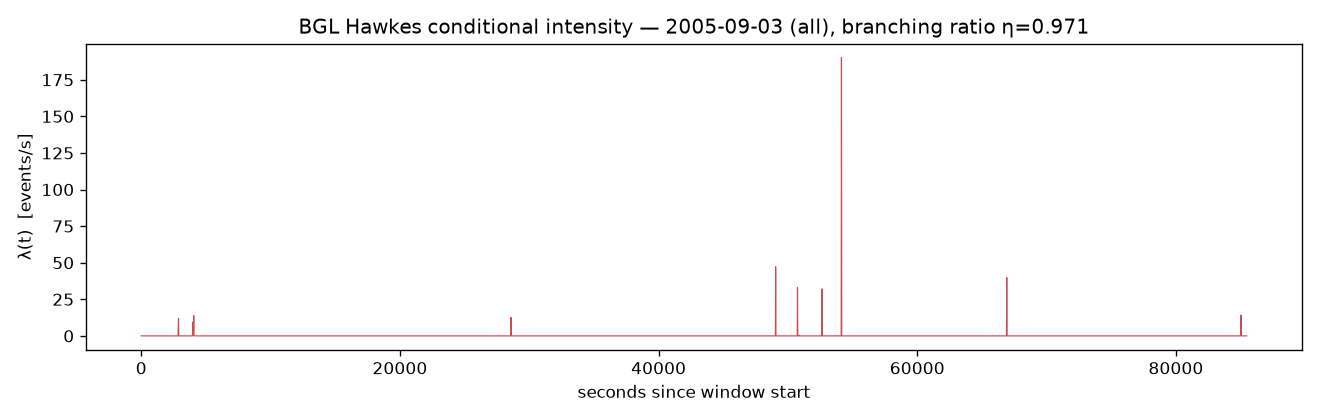
\includegraphics[width=0.7\textwidth]{bgl_hawkes_2005-09-03_all_intensity.png}}{\fbox{figure}}\\[3pt]
\IfFileExists{figures/bgl_hawkes_2005-09-03_all_qq.png}{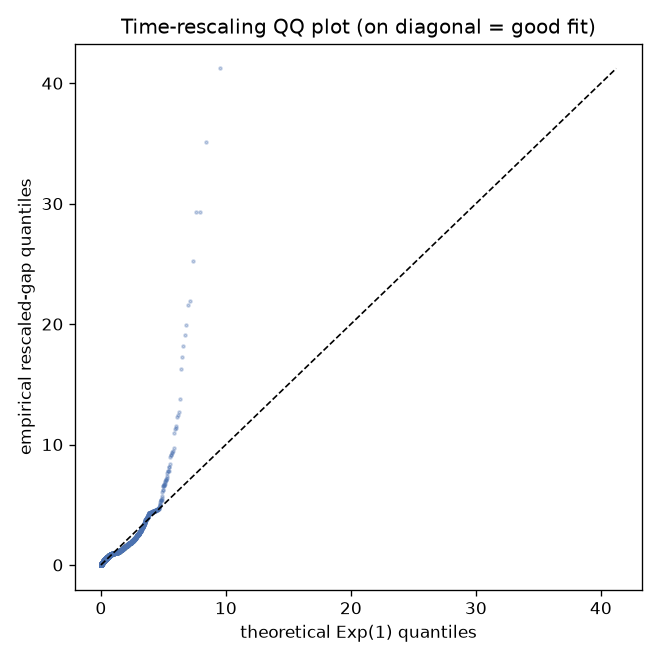
\includegraphics[width=0.38\textwidth]{bgl_hawkes_2005-09-03_all_qq.png}}{\fbox{figure}}
\IfFileExists{figures/bgl_hawkes_2005-06-11_all_qq.png}{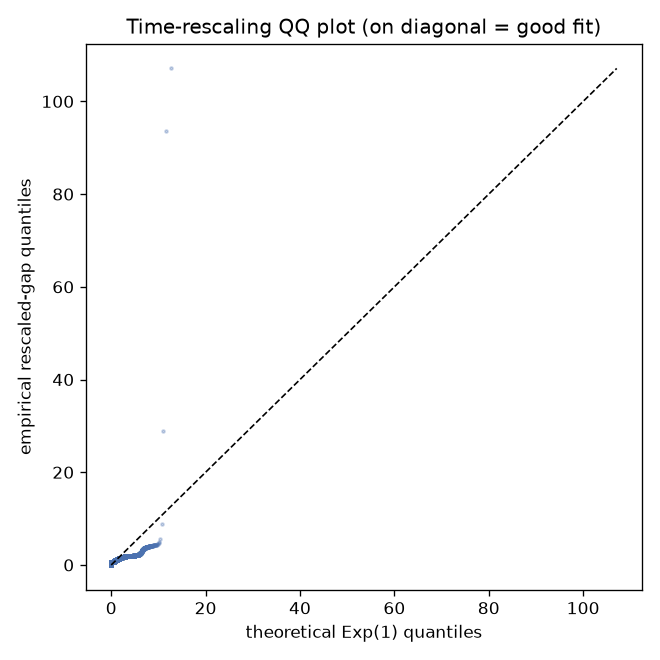
\includegraphics[width=0.38\textwidth]{bgl_hawkes_2005-06-11_all_qq.png}}{\fbox{figure}}
\caption{Top: fitted conditional intensity $\lambda(t)$ on the calm window
---near-zero baseline with self-exciting spikes. Bottom: time-rescaling
QQ-plots against $\mathrm{Exp}(1)$ for the calm (left) and cascade (right)
windows: the body lies on the diagonal, the upper tail departs.}
\label{fig:hawkes}
\end{figure}

\paragraph{Interpretation.} The estimated branching ratio is
\emph{near-critical} on both windows ($\eta\approx0.97$--$1.0$): each event
generates on the order of one direct offspring, i.e.\ the stream operates at
the edge of self-sustaining cascades. This is the project's central
quantitative finding about the data: a precise, validated statement that
sharpens the informal observation ``logs are bursty.'' The time-rescaling
diagnostics simultaneously certify the fit's quality in the bulk (the
QQ body lies on the diagonal; mean rescaled gap $=1.0000$ confirms correct
normalisation) and localise its failure: the upper tail departs upward,
meaning the deepest quiet gaps are longer than a single exponential kernel
allows. The effect is mild on the calm window (KS $0.095$) and severe on the
cascade (KS $0.431$). Mechanistically, after a burst the fitted excitation
predicts continued activity; when silence follows, the integrated intensity
over the gap is inflated. A single time scale cannot fit both tight bursts
and deep lulls---an argument, developed in Chapter~\ref{ch:conclusion}, for
a multi-scale (sum-of-exponentials) kernel. Given the sample sizes, KS
$p$-values are not informative (the test rejects any parametric model at
$n\sim10^5$); the analysis therefore rests on the QQ geometry and the KS
magnitude.

\section{Ablation: do timing features improve detection?}
\label{sec:impl-ablation}
The Hawkes model earns a place in a \emph{detection} pipeline only if its
signal helps. This was tested directly: on 60-second BGL windows, the same
Isolation Forest under the same temporal split was trained on three feature
sets---content only, timing only, and their concatenation
(Section~\ref{sec:method-features}).

\begin{table}[H]
\centering
\caption{Feature ablation on BGL windows (test split, 4.71\% anomalous).}
\label{tab:ablation}
\small
\renewcommand{\arraystretch}{1.2}
\begin{tabular}{@{}l c c c@{}}
\toprule
Feature set & PR-AUC & Precision at recall $0.90$ & False alarms / day \\
\midrule
Content & 0.081 & 0.046 & 114 \\
\rowcolor{remarkbg}\color{good}Timing & \color{good}0.087 & \color{good}0.083 & \color{good}61 \\
Content $+$ timing & 0.090 & 0.071 & 72 \\
Chance & 0.047 & --- & --- \\
\bottomrule
\end{tabular}
\end{table}

\begin{figure}[H]
\centering
\IfFileExists{figures/bgl_timing_ablation.png}{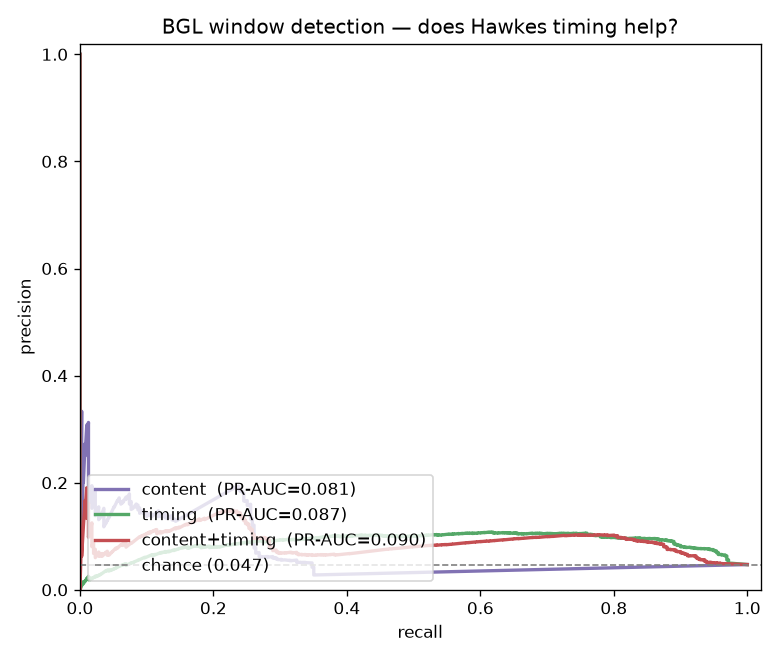
\includegraphics[width=0.55\textwidth]{bgl_timing_ablation.png}}{\fbox{figure}}
\caption{Precision--recall curves for the ablation. The content-only curve
collapses to the chance line at moderate recall; the timing-based curves
retain $\approx2\times$ chance precision across the operating range.}
\label{fig:ablation}
\end{figure}

The result is deliberately reported with both of its faces. In absolute
terms, window-level detection on BGL is \emph{hard}: all feature sets remain
near PR-AUC $0.09$ against a $0.047$ chance level, because a 60-second window
dilutes a handful of alert lines in heavy normal traffic. Relatively,
however, the timing features are the strongest signal available: at recall
$0.90$ they halve the false-alarm rate with respect to content features
($114\to61$/day) and nearly double precision. The self-excitation level thus
carries operationally useful information that count features do not---the
affirmative, if measured, answer to the chapter's question.

\section{Adaptive thresholding under drift}
\label{sec:impl-evt}
The drift decomposition of Section~\ref{sec:impl-detection} identified the
deployment problem: with the threshold fixed once, the autoencoder's
false-alarm rate on HDFS swings from $3{,}664$ to $861{,}686$ per day across
a five-hour test window---at its worst flagging essentially every block.

\paragraph{EVT implementation and a documented failure mode.} The POT
threshold of Equation~\eqref{eq:zq} was implemented with a method-of-moments
GPD estimator (constant-time updates, suitable for streaming) and verified on
simulated data: on stationary streams it holds the target exceedance rate;
on drifting streams it tracks the drift where a fixed threshold fails. On
the real HDFS scores, however, the GPD extrapolation misbehaved---fitted
thresholds could fall below the bulk of the data. The diagnosis is a genuine
property of the data: \textbf{58.7\%} of normal test blocks share a single
\emph{identical} reconstruction-error value (normal HDFS sessions are highly
repetitive, so entire cohorts have byte-identical count vectors). The
resulting score distribution has large atoms, violating the continuity
hypothesis of the Pickands--Balkema--de~Haan theorem
(Section~\ref{sec:theory-evt}). Rather than force the tool, the design
substitutes a \emph{distribution-free} trailing-window quantile on HDFS and
reserves EVT for continuous scores such as the BGL timing features.

\paragraph{Result.} With a target flag rate $q=3\%$, calibrated on the first
20{,}000 test blocks and run over the remaining 152{,}518:

\begin{table}[H]
\centering
\caption{False-alarm stability under drift (HDFS autoencoder scores,
$q=3\%$).}
\label{tab:evt}
\small
\renewcommand{\arraystretch}{1.2}
\begin{tabular}{@{}l c c@{}}
\toprule
 & Fixed threshold & \color{good}Adaptive (trailing quantile) \\
\midrule
False alarms / day (range) & $3{,}664$ -- $861{,}686$ & \ours{$0$ -- $7{,}584$} \\
Flagged fraction & up to $100\%$ & \ours{$\approx2\%$, stable} \\
Recall over the period & $1.00$ & $0.72$ \\
\bottomrule
\end{tabular}
\end{table}

\begin{figure}[H]
\centering
\IfFileExists{figures/hdfs_evt_thresholding.png}{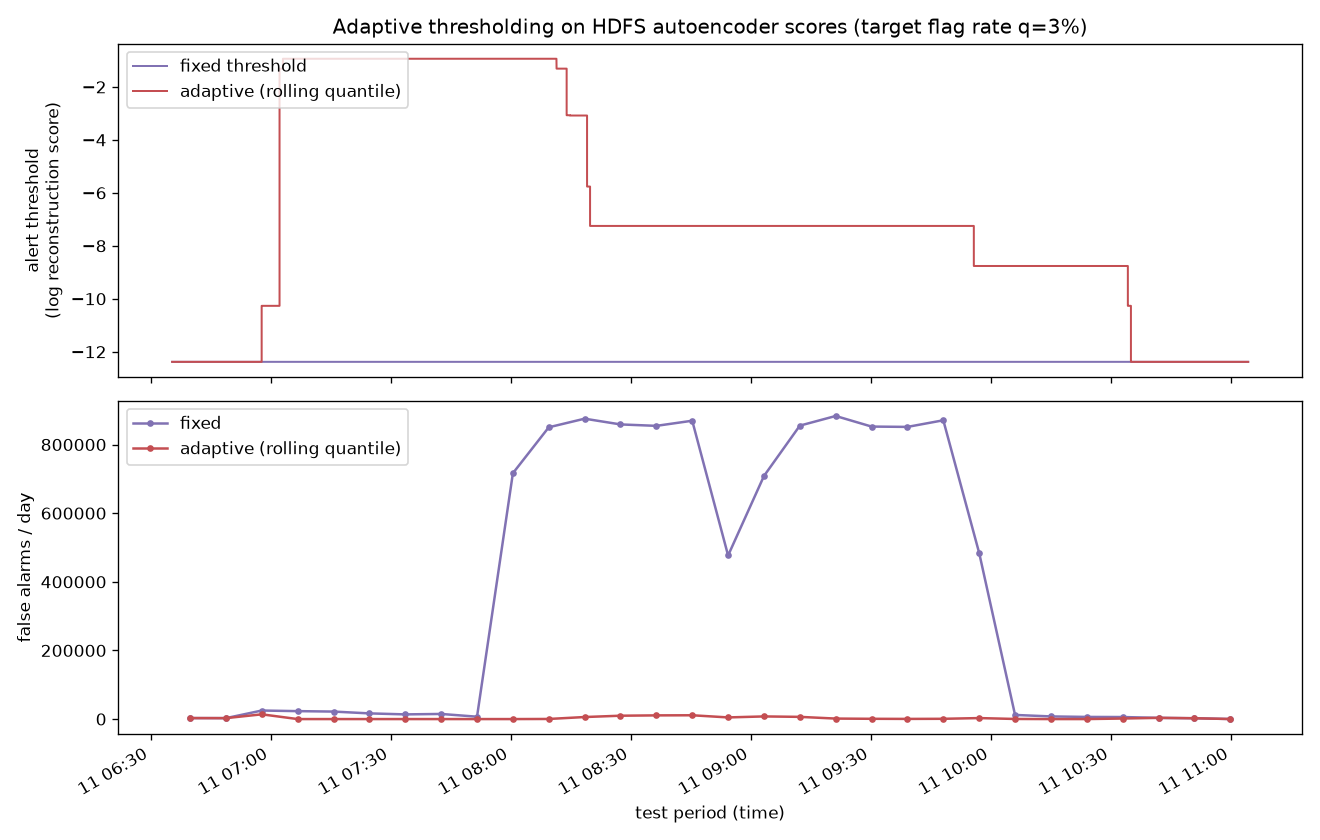
\includegraphics[width=0.78\textwidth]{hdfs_evt_thresholding.png}}{\fbox{figure}}
\caption{Top: fixed versus adaptive threshold against the drifting score
distribution. Bottom: resulting false alarms per day; the fixed threshold
explodes mid-period while the adaptive threshold holds the alert budget.}
\label{fig:evt}
\end{figure}

The adaptive threshold holds the alert volume within budget throughout the
drift, at a transparent cost: when true anomalies exceed the flag budget,
recall falls ($1.00\to0.72$ over the period). The trade-off is not hidden
but exposed as a single tunable parameter $q$---exactly the interface an
operations team needs.

\section{Triage: from alerts to ranked incidents}
\label{sec:impl-triage}
The final analytical stage converts flagged units into analyst-ready
incidents in three deterministic-then-generative steps:
\begin{enumerate}[nosep,leftmargin=1.6em]
  \item \textbf{Deduplication.} Flags with identical signature (entity and
  multiset of templates) are merged, retaining a count---repetition is
  recorded, not re-alerted.
  \item \textbf{Correlation.} Flags close in time are grouped into a single
  incident. The grouping rule is the operational translation of the Hawkes
  analysis: since the stream is near-critically self-exciting, temporally
  clustered anomalies are overwhelmingly cascade members sharing a root
  cause, and belong in one incident.
  \item \textbf{Explanation and ranking.} Each incident is rendered as a
  strictly-typed JSON object (\code{priority}, \code{category},
  \code{summary}, \code{recommended\_action}, \code{explanation}) and the
  incident list is ranked. The explanation backend is pluggable: a
  deterministic rule-based engine (keyword-derived category; priority from
  severity and cascade size) guarantees a self-contained system, while an
  LLM backend (Anthropic API with schema-constrained structured output)
  substitutes richer summaries when credentials are available, falling back
  automatically otherwise. The LLM is invoked once per \emph{incident}, not
  per raw flag; the deterministic reduction upstream is what keeps this
  economical.
\end{enumerate}
On the 200 highest-scoring HDFS test blocks, the agent produced
\textbf{90 incidents} (P1:~13, P2:~53, P3:~2, P4:~22) across data-loss,
replication-failure, and network categories---a $>2\times$ volume reduction
with priorities and actions attached
(Figure~\ref{fig:dash}).

\begin{remark}[Honest note]
In the development environment no LLM credential was available, so the
end-to-end demonstration ran on the rule-based backend; the LLM path is
implemented and tested structurally but was not exercised against a live
model in this report's runs.
\end{remark}

\section{Demonstrator dashboard}
\label{sec:impl-dashboard}
A Streamlit application exposes the pipeline to a non-technical audience in
four views: Detection (metrics and PR curves), Thresholding (the drift
demonstration), Hawkes (fitted intensity and QQ diagnostics), and Incidents
(the ranked incident table with per-incident drill-down). The application
was verified headlessly (HTTP health checks and rendered-page screenshots).

\begin{figure}[H]
\centering
\IfFileExists{figures/dashboard_incidents.png}{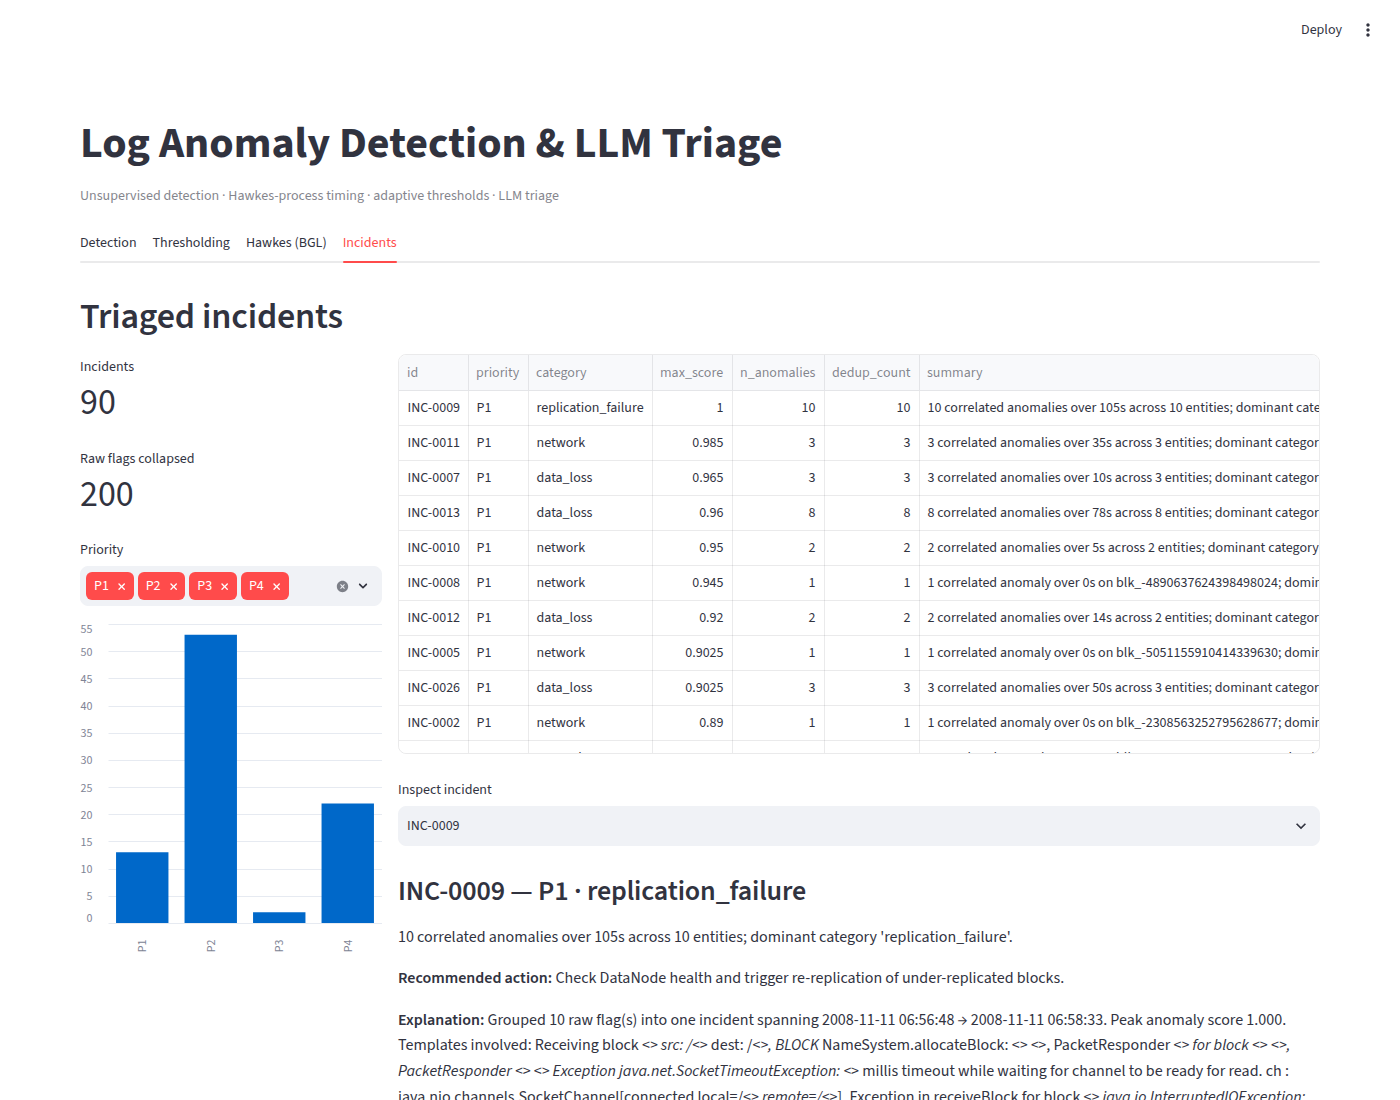
\includegraphics[width=0.8\textwidth]{dashboard_incidents.png}}{\fbox{figure}}
\caption{The Incidents view of the demonstrator: 200 raw flags reduced to 90
ranked incidents with priorities, categories, and recommended actions.}
\label{fig:dash}
\end{figure}

% =============================== CHAPTER 7 ===============================
\chapter{Discussion}
\label{ch:discussion}

\section{Synthesis of results}
Table~\ref{tab:synthesis} consolidates the quantitative outcomes.

\begin{table}[H]
\centering
\caption{Consolidated results of the internship project.}
\label{tab:synthesis}
\small
\renewcommand{\arraystretch}{1.2}
\begin{tabular}{@{}l l@{}}
\toprule
Item & Result \\
\midrule
HDFS parsing & 11.2M lines $\to$ 48 templates (invariant-checked) \\
BGL parsing & 4.71M lines $\to$ 429 templates \\
Detection (HDFS test) & PR-AUC \ours{0.987} vs.\ 0.748 baseline \\
Operational gain & \ours{$\sim$20$\times$} fewer false alarms at recall 0.90 \\
Hawkes branching ratio (BGL) & \ours{$\eta\approx0.97$--$1.0$} (near-critical) \\
Timing-feature effect (BGL) & false alarms \ours{halved} vs.\ content features \\
Thresholding under drift & FA/day swing $\times$235 $\to$ \ours{held near budget} \\
Triage & 200 flags $\to$ \ours{90 ranked incidents} \\
Software quality & 34 automated tests; fully reproducible pipeline \\
\bottomrule
\end{tabular}
\end{table}

\section{Limitations}
\label{sec:limitations}
The following limitations are stated with the same prominence as the
results.
\begin{enumerate}[nosep,leftmargin=1.6em]
  \item \textbf{The HDFS detection figure is a reproduction.} Its value is
  methodological (pipeline validation), not scientific novelty.
  \item \textbf{Absolute detection on BGL windows is weak} (PR-AUC
  $\approx0.09$ against $0.047$ chance). The timing result is a relative
  improvement on a genuinely hard task, and is presented as such.
  \item \textbf{The single-exponential Hawkes kernel is rejected in the
  tail} by its own diagnostic; the branching-ratio estimate on the cascade
  window ($\eta\approx0.9998$) should be read with this misfit in mind.
  \item \textbf{EVT was not applicable to the HDFS scores} (discrete
  atoms); the principled tool was replaced by a distribution-free one there,
  and its intended domain (continuous timing scores) remains to be exercised
  in production-like conditions.
  \item \textbf{The LLM backend was not exercised live} in the reported
  runs.
  \item \textbf{Hyperparameters were fixed a priori} (window length,
  vocabulary size, decay scales, architecture) rather than swept; the
  reported numbers are therefore conservative.
  \item \textbf{Public data stands in for OCP data.} The transfer of these
  methods to an internal log source---with its own formats, volumes, and
  drift regimes---is an engineering exercise that this project prepares but
  does not perform.
\end{enumerate}

\section{Skills developed during the internship}
Beyond the technical artefacts, the internship consolidated: the estimation
and validation of point-process models (likelihood derivation, simulation,
goodness of fit); evaluation methodology for rare-event detection;
extreme-value methods and their hypotheses; applied deep learning for
unsupervised detection; software engineering practice (packaging, automated
testing, reproducibility, version control); and the discipline of
documenting negative findings---arguably the most transferable habit of all
for a career in quantitative research.

% =============================== CHAPTER 8 ===============================
\chapter{Conclusion and perspectives}
\label{ch:conclusion}

\section{Conclusion}
This internship delivered a complete, reproducible log-anomaly pipeline
whose components answer the three structural difficulties of industrial log
analysis identified in Chapter~\ref{ch:company}: unsupervised detection for
the absence of labels, a validated self-exciting timing model for the
cascade structure of incidents, and calibrated alerting plus LLM-assisted
triage for the volume asymmetry. The methodological through-line---prove
estimators on synthetic data, validate on strictly out-of-time data, report
the operationally meaningful metric, and give negative findings first-class
status---is, in the author's view, the internship's most important outcome:
it is what makes each number in this report defensible.

\section{Perspectives}
Four continuations follow naturally from the limitations:
\begin{enumerate}[nosep,leftmargin=1.6em]
  \item \textbf{Multi-scale Hawkes kernels.} Replace the single exponential
  with a sum of exponentials (fast burst + slow relaxation) or a power-law
  kernel, targeting the upper-tail misfit exhibited by time-rescaling.
  \item \textbf{Rescaling residuals as a detector.} The time-rescaling
  transform converts the fitted model into a calibrated ``surprise'' signal;
  large rescaled gaps (or bursts of small ones) are themselves anomaly
  scores, continuous by construction and therefore in EVT's domain.
  \item \textbf{Systematic hyperparameter study} of window length, template
  vocabulary, decay scales, and detector architecture, with the ablation of
  Section~\ref{sec:impl-ablation} as the evaluation harness.
  \item \textbf{Transfer to an internal log source} within the host
  organisation, exercising the LLM triage backend live and measuring analyst
  time saved---the ultimate criterion for the triage layer.
\end{enumerate}

% =============================== BIBLIOGRAPHY ===============================
\begin{thebibliography}{10}
\small
\bibitem{drain} P.~He, J.~Zhu, Z.~Zheng, M.~R.~Lyu. Drain: An Online Log
Parsing Approach with Fixed Depth Tree. \emph{IEEE ICWS}, 2017.
\bibitem{loghub} S.~He, J.~Zhu, P.~He, M.~R.~Lyu. Loghub: A Large Collection
of System Log Datasets for AI-driven Log Analytics. \emph{IEEE ISSRE}, 2023.
\bibitem{loglizer} S.~He, J.~Zhu, P.~He, M.~R.~Lyu. Experience Report:
System Log Analysis for Anomaly Detection. \emph{IEEE ISSRE}, 2016.
\bibitem{deeplog} M.~Du, F.~Li, G.~Zheng, V.~Srikumar. DeepLog: Anomaly
Detection and Diagnosis from System Logs through Deep Learning. \emph{ACM
CCS}, 2017.
\bibitem{loganomaly} W.~Meng et al. LogAnomaly: Unsupervised Detection of
Sequential and Quantitative Anomalies in Unstructured Logs. \emph{IJCAI},
2019.
\bibitem{iforest} F.~T.~Liu, K.~M.~Ting, Z.-H.~Zhou. Isolation Forest.
\emph{IEEE ICDM}, 2008.
\bibitem{hawkes} A.~G.~Hawkes. Spectra of Some Self-Exciting and Mutually
Exciting Point Processes. \emph{Biometrika}, 58(1), 1971.
\bibitem{ogata} Y.~Ogata. On Lewis' Simulation Method for Point Processes.
\emph{IEEE Transactions on Information Theory}, 27(1), 1981.
\bibitem{timerescaling} E.~N.~Brown, R.~Barbieri, V.~Ventura, R.~E.~Kass,
L.~M.~Frank. The Time-Rescaling Theorem and Its Application to Neural Spike
Train Data Analysis. \emph{Neural Computation}, 14(2), 2002.
\bibitem{pickands} J.~Pickands~III. Statistical Inference Using Extreme
Order Statistics. \emph{Annals of Statistics}, 3(1), 1975.
\bibitem{spot} A.~Siffer, P.-A.~Fouque, A.~Termier, C.~Largou\"et. Anomaly
Detection in Streams with Extreme Value Theory. \emph{ACM KDD}, 2017.
\end{thebibliography}

% =============================== APPENDICES ===============================
\appendix
\chapter{Notation}
\begin{table}[H]\centering\small
\renewcommand{\arraystretch}{1.2}
\begin{tabular}{@{}c l@{}}
\toprule
Symbol & Meaning \\
\midrule
$\lambda(t)$ & conditional intensity of a point process \\
$\mu,\alpha,\beta$ & Hawkes background rate, excitation jump, decay rate \\
$\eta=\alpha/\beta$ & branching ratio (mean direct offspring per event) \\
$\Lambda(t)$ & compensator $\int_0^t\lambda(s)\,ds$ \\
$\Delta\tau_i$ & rescaled inter-event increment ($\mathrm{Exp}(1)$ under a correct model) \\
$(\gamma,\sigma)$ & GPD shape and scale \\
$z_q$ & threshold exceeded with target probability $q$ \\
$x_u,\ y_u,\ s(u)$ & feature vector, latent label, anomaly score of unit $u$ \\
\bottomrule
\end{tabular}
\end{table}

\chapter{Reproducibility}
All code, tests, figures, and this report's sources are versioned in the
project repository. The pipeline is reproduced end to end by the following
sequence (Python $\geq$3.10):
\begin{quote}\small\ttfamily
pip install -r requirements.txt \&\& pip install -{}-no-deps logparser3 \&\& pip install -e .\\[2pt]
python scripts/download.py -{}-dataset HDFS -{}-full\\
python scripts/parse.py -{}-dataset HDFS -{}-input data/raw/HDFS.log\\
python scripts/build\_features.py -{}-input data/interim/HDFS.log\_parsed.csv
-{}-labels data/raw/anomaly\_label.csv\\
python scripts/run\_baseline.py \quad\#\ Isolation Forest\\
python scripts/train\_autoencoder.py\\
python scripts/run\_evt.py -{}-q 0.03\\
python scripts/run\_triage.py -{}-top 200\\[2pt]
python scripts/download.py -{}-dataset BGL -{}-full\\
python scripts/parse.py -{}-dataset BGL -{}-input data/raw/BGL.log\\
python scripts/fit\_hawkes.py -{}-start 2005-06-11 -{}-hours 24 -{}-stream all\\
python scripts/bgl\_experiment.py -{}-window 60 -{}-top-k 50\\[2pt]
streamlit run app/dashboard.py
\end{quote}
The automated test suite is run with \code{python -m pytest tests/}.

\end{document}
